\documentclass[11pt]{article}
%--------------------BLOQUE DE FORMATO--------------------%
\usepackage[a4paper,includehead,includefoot, left=2cm,top=1.2cm,right=2cm,bottom=1.5cm,headheight=28pt]{geometry} %margenes.
%--------------------FIN DE BLOQUE DE FORMATO--------------------%

%--------------------CONFIGURACION DE IDIOMA--------------------%
\usepackage[spanish,es-tabla]{babel} % pone el idioma en español, es-tabla para Tabla en lugar de Cuadro
\usepackage[utf8]{inputenc} % Codificación de entrada, carácteres acentuados, ñ
\usepackage[T1]{fontenc} % Codificación de fuente, habilita caracteres no latinos
\usepackage{lmodern} % Fuente compatible
%--------------------FIN DE CONFIGURACION DE IDIOMA--------------------%

%-----------------PAQUETES NUESTROS-----------------------%

\usepackage[center]{caption} %permite modificar el formato de los caption para tablas/figuras
\usepackage[colorlinks=false,linkcolor=black]{hyperref} %pone vinculos en el indice y en las referencias
\usepackage{adjustbox}
\usepackage{amsmath,amsfonts,amssymb,amscd}  %para ecuaciones
\usepackage{array} %permite escribir en columnas sin ser una tabla, por ejemplo, matrices
\usepackage{bm} %permite usar simbolos matematicos en negrita
\usepackage{bookmark}
\usepackage{booktabs} %modificación de las lineas en las tablas
\usepackage{cancel} %permite tachar terminos en ecuaciones
\usepackage{chemfig} %permite realizar representaciones en 2D de estructuras químicas
\usepackage{circuitikz}
\usepackage{comment} %para comentar grandes partes de codigo, usar \begin{comment}
\usepackage{csquotes}
\usepackage{dsfont} %letras mayúsculas para conjuntos (Ej: Naturales)
\usepackage{enumerate} %permite hacer listas numeradas y por niveles
\usepackage{etoolbox} %crea condicionales, puedo tener dos PDFs distintos desde un solo archivo fuente
\usepackage{fancyhdr} % Modificar encabezados y pies de paginas.
\usepackage{float} %para el float H en tablas.
\usepackage{graphicx} %para insertar graficos e imagenes.
\usepackage{mwe} %para usar example-image como placeholder de simulaciones
\usepackage{lipsum} %introduce bloques de texto random, usado para tests
\usepackage{listings} %para ingresar codigos de MATLAB, Python, Fortran, etc
\usepackage{mathrsfs} %letras mayúsculas especiales, cursiva, gotica, etc
\usepackage{multicol}
\usepackage{multirow} %filas múltiples en tablas
\usepackage{nicefrac} %Permite escribir fracciones en el medio del texto de una forma elegante \nicefrac{a}{b}
\usepackage{parskip} %modificación de sangría
\usepackage{setspace} %permite cambiar espacio entre lineas
\usepackage{stackrel} %Permite escribir cosas arriba o abajo de otras
\usepackage{steinmetz} %mejora la forma de escribir numeros complejos
\usepackage{subfigure}
\usepackage{tabularx}
\usepackage{tikz}
\usepackage{wrapfig}
\usepackage{xcolor} %permite escribir texto en color

%-------------------- Bibliografía --------------------%
\usepackage[backend=biber,style=ieee]{biblatex} %agrega bibliografía al documento
\addbibresource{Preambulo/Bibliografia.bib}

%--------------------Titulos y enumeración de secciones--------------------%
%titulos de secciones y subsecciones.
\makeatletter
\renewcommand\section{\@startsection{section}{1}{\z@}{-3.5ex\@plus-1ex\@minus-.2ex}{2.3ex\@plus.2ex}{\normalfont\Large\bfseries}}
\renewcommand\subsection{\@startsection{subsection}{2}{\z@}{-3.25ex\@plus-1ex\@minus-.2ex}{1.5ex\@plus.2ex}{\normalfont\large\bfseries\raggedright}}
\renewcommand\subsubsection{\@startsection{subsubsection}{3}{\z@}{-3.25ex\@plus-1ex\@minus-.2ex}{1.5ex\@plus.2ex}{\normalfont\normalsize}}
\makeatother

%enumeración de secciones y subsecciones.
\renewcommand{\labelenumi}{\arabic{section}.\arabic{enumi}}
\renewcommand{\labelenumii}{\arabic{section}.\arabic{enumi}.\arabic{enumii}}
\renewcommand{\labelenumiii}{\arabic{section}.\arabic{enumi}.\arabic{enumii}.\arabic{enumiii}}
\renewcommand{\labelenumiv}{\arabic{section}.\arabic{enumi}.\arabic{enumii}.\arabic{enumiii}.\arabic{enumiv}}

\renewcommand{\thefigure}{\arabic{section}.\arabic{figure}}  %definición enumeración de figuras.

\renewcommand{\thesubfigure}{(\alph{subfigure})} %modificación enumeración de subfiguras.

\renewcommand{\thetable}{\arabic{section}.\arabic{table}} %definición enumeración de tablas.

\setcounter{tocdepth}{2} %hasta que nivel aparece en el índice
\setcounter{secnumdepth}{3} %hasta que nivel se enumera
%niveles 1:section, 2:subsection, 3:subsubsection...

%--------------------CONFIGURACION LISTING--------------------%
\usepackage[scaled=0.85]{beramono}            % load a nice TT font
\definecolor{codegreen}{rgb}{0,0.6,0}
\definecolor{codegray}{rgb}{0.5,0.5,0.5}
\definecolor{codepurple}{rgb}{0.58,0,0.82}
\definecolor{backcolour}{rgb}{0.95,0.95,0.92}

\lstdefinestyle{mystyle}{
    backgroundcolor=\color{backcolour},   
    commentstyle=\color{codegreen},
    keywordstyle=\color{magenta},
    numberstyle=\tiny\color{codegray},
    stringstyle=\color{codepurple},
    basicstyle=\ttfamily\footnotesize,
    breakatwhitespace=false,         
    breaklines=true,                 
    captionpos=b,                    
    keepspaces=true,                 
    numbers=left,                    
    numbersep=5pt,                  
    showspaces=false,                
    showstringspaces=false,
    showtabs=false,                  
    tabsize=2
}

\newcommand{\blank}{\mathord{\rule{2.5em}{0.4pt}}}

\lstset{style=mystyle}
%--------------------FIN CONFIGURACION LISTING--------------------%


%---------------- INICIO DEL DOCUMENTO ----------------%
\begin{document}
\def\declvar#1#2{%
   \ifx#1\undefined{}
       \newtoks#1%
   \fi
   #1={#2}}%

% Variables
\declvar\titulo{Trabajo Práctico N\textsuperscript{o} 3}
\declvar\nombreTP{Respuesta en Frecuencia y Estabilización de Circuitos Realimentados}
\declvar\dia{27}
\declvar\mes{Mayo}
\declvar\ano{2026}

% Constantes
\declvar\grupo{}
\declvar\materia{25.55 - Microelectrónica}
\declvar\profesores{Juan Manuel Cesaretti, Eduardo Diocles Baez y Ezequiel David Rubinsztain}

% Estudiante A
%\declvar\nomEstudianteA {BOTTINELLI, LUCA}
%\declvar\legajoEstudianteA {61270}
%\declvar\mailEstudianteA {lbottinelli@itba.edu.ar}
% Estudiante B
%\declvar\nomEstudianteB {GOMEZ, JOAQUIN}
%\declvar\legajoEstudianteB {62116}
%\declvar\mailEstudianteB {joagomez@itba.edu.ar}
% Estudiante C
%declvar\nomEstudianteC {KRAMER, CRISTOBAL }
%\declvar\legajoEstudianteC {62902}
%\declvar\mailEstudianteC {ckramerrodrigo@itba.edu.ar}
% Estudiante A
\declvar\nomEstudianteA{BELSITO, RAMIRO}
\declvar\legajoEstudianteA{62641}
\declvar\mailEstudianteA{rabelsito@itba.edu.ar}
%-------------------- PORTADA --------------------%
\def\declvar#1#2{%
   \ifx#1\undefined{}
       \newtoks#1%
   \fi
   #1={#2}}%

% Variables
\declvar\titulo{Trabajo Práctico N\textsuperscript{o} 3}
\declvar\nombreTP{Respuesta en Frecuencia y Estabilización de Circuitos Realimentados}
\declvar\dia{27}
\declvar\mes{Mayo}
\declvar\ano{2026}

% Constantes
\declvar\grupo{}
\declvar\materia{25.55 - Microelectrónica}
\declvar\profesores{Juan Manuel Cesaretti, Eduardo Diocles Baez y Ezequiel David Rubinsztain}

% Estudiante A
%\declvar\nomEstudianteA {BOTTINELLI, LUCA}
%\declvar\legajoEstudianteA {61270}
%\declvar\mailEstudianteA {lbottinelli@itba.edu.ar}
% Estudiante B
%\declvar\nomEstudianteB {GOMEZ, JOAQUIN}
%\declvar\legajoEstudianteB {62116}
%\declvar\mailEstudianteB {joagomez@itba.edu.ar}
% Estudiante C
%declvar\nomEstudianteC {KRAMER, CRISTOBAL }
%\declvar\legajoEstudianteC {62902}
%\declvar\mailEstudianteC {ckramerrodrigo@itba.edu.ar}
% Estudiante A
\declvar\nomEstudianteA{BELSITO, RAMIRO}
\declvar\legajoEstudianteA{62641}
\declvar\mailEstudianteA{rabelsito@itba.edu.ar}

\begin{titlepage}
    \begin{figure}[t!]
    \centering
    
\includegraphics[scale=0.1]{Imagenes/LOGO ITBA.png}
    \end{figure}
    
    \centering
    %{\Large{Trabajo Practico N° 3}\par}
    %\vspace{0.25cm}
    {\large{\the\materia}\par}
    \vspace{0.3cm}
    {\bfseries\Huge{\the\titulo}\par}
    \vspace{0.5cm}
    {\huge{\the\nombreTP}\par}
    \vspace{.5cm}
    {\large{\the\grupo}\par}
    \vspace{2cm}
    {\large{ \slshape
    \begin{tabbing}

        \the\nomEstudianteA \quad\quad\quad\= \the\legajoEstudianteA \quad\quad\= \href{mailto:	\the\mailEstudianteA}{\texttt{\the\mailEstudianteA}} \\
        \\
        %\the\nomEstudianteB \> \the\legajoEstudianteB \> \href{mailto:	\the\mailEstudianteA}{\texttt{\the\mailEstudianteB}} \\
        \\
        %\the\nomEstudianteC \> \the\legajoEstudianteC \> \href{mailto:	\the\mailEstudianteA}{\texttt{\the\mailEstudianteC}} \\
        \\
        %\the\nomEstudianteD \> \the\legajoEstudianteD \> \href{mailto:	\the\mailEstudianteA}{\texttt{\the\mailEstudianteD}} \\

    \end{tabbing}
    }\par}
 
    \vspace{4cm}
    {\large{Profesores: \the\profesores}\par}
    {\large{Fecha de entrega: \the\dia \space de \the\mes \space de \the\ano}\par}
    
\end{titlepage}
\newpage

%-------------------- INDICES --------------------%
\newpage
\pagestyle{empty}
\renewcommand{\contentsname}{{\huge Índice}}
\tableofcontents

%---------------- DESARROLLO ----------------%
\lhead{\the\materia}
\chead{
\includegraphics[scale=0.02]{Imagenes/LOGO ITBA.png}}
\rhead{\the\grupo}

%---------------- Info de Pagina ----------------%
\newpage
\pagestyle{fancy} %activa encabezado y pie de pagina

\setcounter{page}{1} %empezar numeración desde está pagina
\setcounter{equation}{0} %empezar numeración desde 1 para ecuaciones
\setcounter{figure}{0} %empezar numeración desde 1 para figuras
\setcounter{table}{0} %empezar numeración desde 1 para tablas

%\label{sec: label de la seccion} %los labels tambien funcionan con secciones

%---------------- Introducción ---------------%
\section{Introducción}
El presente informe aborda el análisis de estabilidad y respuesta en frecuencia de circuitos realimentados propuestos en el Trabajo Práctico Nro. 3. En particular, se estudia el circuito de la figura 1 para determinar la posición de sus polos y comparar el resultado teórico con la simulación. Luego se desarrolla el diseño de la capacidad de compensación C1 para obtener un margen de fase de $45^\circ$ con $\beta=1$ y se evalúa la estabilización mediante efecto Miller y ``nulling resistor''.

A continuación, se analiza el amplificador operacional de la figura 2 utilizado como buffer de tensión, con atención a la respuesta al escalón y la obtención de un margen de fase de $60^\circ$. También se destaca la alternativa de obtención de ganancia $\text{AOL}\beta$ descrita en la figura 3, manteniendo la polarización de DC.

Cada sección incluye los resultados teóricos principales, los espacios reservados para las fórmulas y resultados numéricos, y los placeholders para las capturas de las simulaciones en LTspice.


%---------------- 1ra Seccion ----------------%
\section{Ejercicio 1}
\label{sec:ejercicio1}
\subsection{Circuito de la figura 1}
El primer ejercicio se centra en el circuito de la figura 1. Se realiza el cálculo de los polos a partir de la función de transferencia del lazo abierto y se contrasta esta ubicación con los resultados obtenidos en simulación.

\subsubsection{Cálculo teórico de los polos}
A partir del modelo del circuito se obtiene la expresión característica. 
Función transferencia del lazo abierto:
\begin{equation}
    H_{(s)} = 20\frac{\mu A}{V} \cdot \frac{R_1}{1 + sC_1R_1} \cdot 10 \frac{\mu A}{V} \cdot \frac{R_2}{1 + sC_2R_2}
\end{equation}
Ubicación de los polos:
\begin{equation}
    s_1 = -\frac{1}{C_1R_1} \Rightarrow f_1 = 63.661\,\text{kHz}, \quad s_2 = -\frac{1}{C_2R_2} \Rightarrow f_2 = 1.591\,\text{MHz}
\end{equation}

\subsubsection{Contraste con simulación}
La comparación entre los valores teóricos y los extraídos de la respuesta en frecuencia permite verificar la validez del modelo y detectar posibles discrepancias debidas a la modelización del op-amp.

\begin{figure}[H]
    \centering
    
\includegraphics[width=0.9\textwidth]{example-image}
    \caption{Respuesta en frecuencia del circuito de la figura 1 (placeholder: example-image.png).}
    \label{fig:sim1}
\end{figure}

\vspace{2em}

\subsubsection{Resultados}
\noindent\textbf{Polos teóricos:}
\vspace{3em}

\noindent\textbf{Polos simulados:}
\vspace{3em}

\noindent\textbf{Comentarios sobre la comparación:}
\vspace{3em}


%---------------- 2da Seccion ----------------%
\section{Ejercicio 2}
\label{sec:ejercicio2}
\subsection[Diseño para margen de fase de 45° con beta=1]{Diseño para margen de fase de $45^\circ$ con $\beta=1$}
En esta sección se desarrolla la modificación del circuito de la figura 1 para que el sistema realimentado presente un margen de fase de $45^\circ$ con $\beta=1$.

\subsubsection[Valor de C1 para 45°]{Valor de C1 para $45^\circ$}

A partir de la modificación del circuito sin el agregado de un capacitor de compensación.
Para evitar oscilaciones en el sistema realimentado, se busca asegurar un margen de fase positivo y suficientemente grande. 
En este caso, se fuerza la frecuencia de cruce de ganancia a coincidir con la frecuencia del segundo polo:

\[
\omega_c=\omega_{p2}
\]

Si el primer polo se ubica suficientemente por debajo de la frecuencia de cruce, idealmente al menos una década antes, su contribución de fase en \(\omega_c\) será aproximadamente:

\[
\phi_1(\omega_c)\approx -90^\circ
\]

Por otro lado, como la frecuencia de cruce coincide con el segundo polo, la contribución de fase del segundo polo será:

\[
\phi_2(\omega_c)=-45^\circ
\]

Por lo tanto, la fase total de la ganancia de lazo abierto en la frecuencia de cruce será aproximadamente:

\[
\phi(\omega_c)\approx -90^\circ-45^\circ=-135^\circ
\]

El margen de fase resulta entonces:

\[
PM = 180^\circ + \phi(\omega_c)
\]

\[
PM \approx 180^\circ - 135^\circ = 45^\circ
\]

De esta manera, al elegir \(C_1\) de forma tal que \(\omega_c=\omega_{p2}\), y verificando que \(\omega_{p1}\ll \omega_c\), se obtiene un margen de fase cercano a \(45^\circ\), evitando que el sistema realimentado oscile.

\vspace{3em}

\subsubsection{Estabilización por efecto Miller}
Utilizando el efecto Miller se propone una red de compensación que cancela el cero de signo positivo y estabiliza el sistema.
\vspace{3em}

\subsection*{Eliminación del cero de semiplano derecho mediante nulling resistor}

Al compensar el sistema con un capacitor de Miller \(C_c\) conectado entre la entrada y la salida de la segunda etapa, aparece un camino directo de \textit{feedforward} entre ambos nodos. Este camino permite que parte de la señal llegue a la salida sin pasar por la transconductancia de la segunda etapa, \(g_{m2}\).

La corriente generada por la segunda etapa es:

\[
i_{gm2}=g_{m2}v_a
\]

mientras que la corriente que circula por el capacitor de compensación es:

\[
i_{C_c}=sC_c(v_a-v_o)
\]

Este camino capacitivo introduce un cero en la función de transferencia. Sin resistencia serie, es decir para \(R_z=0\), el cero se ubica aproximadamente en:

\[
s_z=+\frac{g_{m2}}{C_c}
\]

Por lo tanto, el cero queda en el semiplano derecho. Este cero es indeseado porque, aunque incrementa la pendiente de magnitud como un cero convencional, introduce atraso de fase. Es decir, su contribución de fase tiende a:

\[
\phi_z \rightarrow -90^\circ
\]

reduciendo el margen de fase del sistema realimentado.

Para eliminar este cero, se agrega una resistencia \(R_z\) en serie con el capacitor de Miller. La impedancia de compensación pasa a ser:

\[
Z_c = R_z+\frac{1}{sC_c}
\]

Con esta resistencia serie, la posición del cero queda dada por:

\[
s_z=
\frac{g_{m2}}{C_c(1-g_{m2}R_z)}
\]

A partir de esta expresión se observa que:

\[
R_z=0
\quad \Rightarrow \quad
s_z=+\frac{g_{m2}}{C_c}
\]

es decir, el cero queda en el semiplano derecho.

Si se elige:

\[
R_z>\frac{1}{g_{m2}}
\]

entonces:

\[
1-g_{m2}R_z<0
\]

y el cero se traslada al semiplano izquierdo.

Sin embargo, si se quiere eliminar el cero del rango de frecuencias de interés, se impone:

\[
R_z=\frac{1}{g_{m2}}
\]

En ese caso:

\[
1-g_{m2}R_z=0
\]

por lo tanto:

\[
s_z \rightarrow \infty
\]

Esto significa que el cero queda desplazado a frecuencia infinita y desaparece de la respuesta del sistema en el rango útil.

Físicamente, la condición

\[
\boxed{R_z=\frac{1}{g_{m2}}}
\]

hace que la corriente directa que circula por el capacitor de Miller se cancele con la corriente generada por la transconductancia de la segunda etapa. De esta forma se anula el camino de \textit{feedforward} responsable del cero en el semiplano derecho.

En este circuito:

\[
g_{m2}=10\frac{\mu A}{V}=10\ \mu S
\]

Luego:

\[
R_z=\frac{1}{10\times 10^{-6}}
\]

\[
\boxed{R_z=100\ k\Omega}
\]

Por lo tanto, el nulling resistor necesario para eliminar el cero de semiplano derecho debe ser:

\[
\boxed{R_z=\frac{1}{g_{m2}}=100\ k\Omega}
\]
\noindent\textbf{Capacitor CM experimental:}
\vspace{3em}

$C_m = 0.88pF$

\subsubsection{Simulación de la compensación}

\begin{figure}[H]
    \centering
    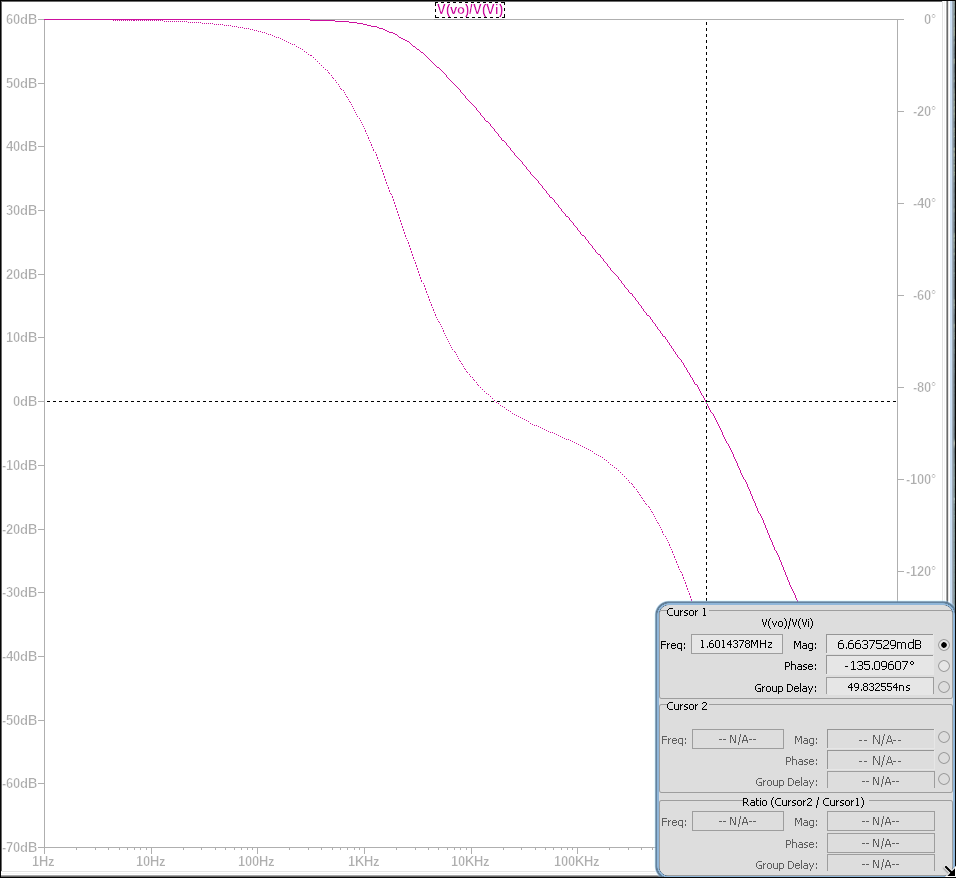
\includegraphics[width=0.9\textwidth]{Imagenes/PMSim14pSinCircuito.png}
    \caption{Simulación de la compensación con efecto Miller}
    \label{fig:sim2}
\end{figure}

\vspace{2em}

\noindent\textbf{Comentarios sobre la estabilidad:}
\vspace{3em}

Este capacitor permite, sin modificar el diseño del circuito aprovechar la alta ganancia en la etapa para evitar la oscilación, obteniendo el comportamiento deseado.

%---------------- 3ra Seccion ----------------%
\section{Ejercicio 3}
\label{sec:ejercicio3}
\subsection{Circuito buffer de la figura 2}
El tercer ejercicio evalúa el amplificador operacional utilizado como buffer de tensión, y su ajuste para lograr un margen de fase de $60^\circ$.

\subsubsection{Respuesta al escalón}
Se simula la respuesta temporal del buffer ante una señal escalón y se analizan los parámetros de overshoot y tiempo de establecimiento.

\begin{figure}[H]
    \centering
    
\includegraphics[width=0.9\textwidth]{example-image}
    \caption{Respuesta al escalón del buffer de la figura 2 (placeholder: example-image.png).}
    \label{fig:sim3}
\end{figure}

\vspace{2em}

\noindent\textbf{Parámetros temporales extraídos:}
\vspace{3em}

\subsubsection{Diseño para PM = $60^\circ$}
Se describe el procedimiento para obtener experimentalmente el valor de CM y del nulling resistor que permiten alcanzar un margen de fase de $60^\circ$.

\vspace{3em}

\noindent\textbf{Valores ajustados:}
\vspace{3em}

\subsubsection{Contraste teórico-experimental}
Se comparan las posiciones de los polos calculadas teóricamente con las obtenidas en la simulación real del circuito.

\vspace{2em}

\noindent\textbf{Polos teóricos:}
\vspace{3em}

\noindent\textbf{Polos simulados:}
\vspace{3em}

\subsection{Alternativa de polarización de la figura 3}
Se incluye una breve referencia a la alternativa de obtención de la ganancia $\text{AOL}\beta$ manteniendo la polarización de DC, según lo indicado en la figura 3.

\vspace{3em}

\noindent\textbf{Observaciones sobre la alternativa de polarización:}
\vspace{3em}


%----------------- Conclusión ----------------%
\section{Conclusión}
El cierre del informe resume los resultados principales del análisis de estabilidad y respuesta en frecuencia de los circuitos propuestos.

\noindent\textbf{Resumen de los hallazgos principales:}
\vspace{3em}

\noindent\textbf{Cumplimiento de los objetivos del TP:}
\vspace{3em}

\noindent\textbf{Recomendaciones finales:}
\vspace{3em}


%---------------- Anexo ----------------%
%\newpage
%\section{Anexo}
%\input{Secciones/anexo}

%---------------- Bibliografía ----------------%
%\printbibliography

%---------------- Componentes ----------------%
\newpage
\section{Templates}
% -------- TABLAS ---------------
\subsection{Tablas}
\begin{table}[H]
    \centering
    \begin{tabular}{l|c|c} \hline
     Columna 0 & Columna 1 & Columna 2  \\ \hline
    0 & 1 & 2  \\ 
    0 & 1 & 2 \\ \hline
    \end{tabular}
    \caption{Pie de tabla}
    \label{tab:tabla simple}
\end{table}



% ---------- FOTOS --------------
\subsection{Fotos}
% 1. Simple
\subsubsection{Foto Simple}
\begin{figure}[H]
    \centering
    
\includegraphics[width=0.5\linewidth]{Imagenes/example-image.png}
    \caption{Foto simple}
    \label{fig:foto simple}
\end{figure}

% 2. Varias horizontales
\subsubsection{Fotos Horizontales}
\begin{figure}[H]
    \subfigure[Foto 1]{
    
\includegraphics[width=0.3\textwidth]{Imagenes/example-image.png}}
    \subfigure[Foto 2]{
    
\includegraphics[width = 0.3\textwidth]{Imagenes/example-image.png}}
    \subfigure[Foto 3]{
    
\includegraphics[width = 0.3\textwidth]{Imagenes/example-image.png}}
    \label{fig:multi Fotos}
\end{figure}

% 3. Varias verticales
\subsubsection{Fotos Verticales}
\begin{figure}[H]
    \centering
    
\includegraphics[width=0.5\linewidth]{Imagenes/example-image.png}
    
\includegraphics[width=0.5\linewidth]{Imagenes/example-image.png}
    \caption{2 fotos verticales}
    \label{fig:fotos verticales}
\end{figure}

% 4. Grilla de Fotos
\subsubsection{Fotos en grilla}
\begin{figure}[H]
        \subfigure[Caption 1]{
            
\includegraphics[width=.48\linewidth]{Imagenes/example-image.png}
            \label{subfig:a}
        }\hfill
        \subfigure[Caption 2]{
            
\includegraphics[width=.48\linewidth]{Imagenes/example-image.png}
            \label{subfig:b}
        }\\
        \subfigure[Caption 3]{
            
\includegraphics[width=.48\linewidth]{Imagenes/example-image.png}
            \label{subfig:c}
        }\hfill
        \subfigure[Caption 4]{
            
\includegraphics[width=.48\linewidth]{Imagenes/example-image.png}
            \label{subfig:d}
        }
        \caption{Caption}
        \label{fig: grilla de fotos}
    \end{figure}

% -------------- Texto en dos columnas -------------
\subsection{Texto en Columnas}
\setlength{\columnsep}{1cm}
\begin{multicols}{2}
Lorem ipsum dolor sit amet, consectetur adipiscing elit. Proin tristique aliquam sapien pellentesque viverra. Proin in ex libero. Etiam cursus et metus ut porttitor. Nunc sit amet rhoncus velit. Nunc eu pharetra sapien. In ultricies tellus a sapien placerat, quis commodo sem consequat. Sed non felis sagittis, maximus felis dictum, scelerisque eros. Nunc in aliquet lacus. Ut consectetur odio purus. Integer sed erat quis mi vulputate molestie. Etiam viverra sapien tincidunt turpis pulvinar blandit. Nullam pharetra bibendum ligula, vitae dictum est sagittis ut. Suspendisse convallis commodo diam at elementum.
\end{multicols}

% ------------ Ecuaciones -----------------------

% Sistema de ecuaciones
\subsection{Ecuaciones}
\begin{equation}
    \begin{cases}
        2x+y=1 \\
        y+2=3
    \end{cases} \longrightarrow x=0 \wedge y=1
\end{equation} 


% Ecuaciones alineadas
\begin{equation}
    \begin{gathered}
        H(s) = \frac{1}{\frac{1}{sRC}} \\
        H(s)= sRC
    \end{gathered}
\end{equation}

% Ecuaciones alineadas por el igual
\begin{equation}
    \begin{split}
        H(s) &= \frac{1}{\frac{1}{sRC}} \\
             &= sRC
    \end{split}
\end{equation}



% Ecuaciones sin número
$$H(s)= sRC$$




% ---------------- Citas y Links -----------------
\subsection{Citas y Links}

Dirac dijo esto. \cite{dirac}

\href{http://www.overleaf.com}{Esto tiene un hipervínculo}


% ----------------- Bloque de código -------------------
\subsection{Código}
\begin{lstlisting}
# Bloque de codigo
...
...
print('Hello World!)
\end{lstlisting}





\end{document}
